\documentclass{beamer}

%\usetheme[framenumber,totalframenumber]{UniversiteitGent}
%\usetheme[faculty=di,framenumber,totalframenumber]{UniversiteitGent}
%\usetheme[faculty=we,usecolors,framenumber,totalframenumber]{UniversiteitGent}
%\usetheme[language=english,framenumber,totalframenumber]{AlleghenyCollege}
\usetheme{AnnArbor}
\usecolortheme{dove}

\title{CMPSC 390 \\ Security. Community and Regulations.}
\author{Janyl Jumadinova \\ $ $ \\ Credit: Authors of ``Mastering Bitcoin" and ``Bitcoin and Cryptocurrency Technologies"}
\date{February 2, 2021}

\long\def\omitit#1{}

\usepackage{hyperref}
\hypersetup{
    colorlinks=true,
    linkcolor=blue,
    filecolor=magenta,      
    urlcolor=cyan,
}

\begin{document}

\begin{frame}
  \titlepage
\end{frame}

%%%%%%%%%%%% Slide %%%%%%%%%%%%%%%%%%%%%%%%%%%%%%%%%%%%%%%%%%%%%%%%%%%
\begin{frame}
  \frametitle{Security, Chapter 11 in MB}
	\begin{itemize}
		\item Can be backed up and stored in multiple copies. \pause
		\item Decentralization is important for security. \pause
		\item Responsibility and control is in the hands of the users. \pause
		\item Bitcoin is not based on \textcolor{brown}{Root of Trust} security architecture,which is designed as a series of concentric circles. \pause
		\item Genesis block is the root of trust, a chain of trust built up to the current block. \pause
		\item \emph{Balancing risk}: storage, multisig, diversification, survivability.
	\end{itemize}
\end{frame}
%%%%%%%%%%%% Slide %%%%%%%%%%%%%%%%%%%%%%%%%%%%%%%%%%%%%%%%%%%%%%%%%%%
\begin{frame}
  \frametitle{Consensus in Bitcoin}
 	\centering
	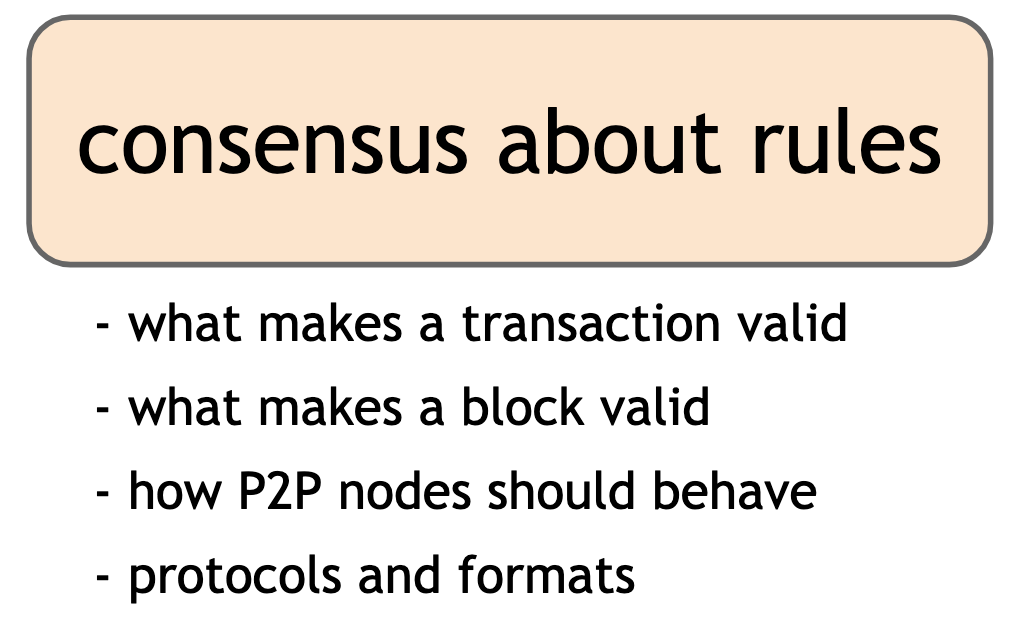
\includegraphics[scale=0.28]{rules}
\end{frame}
%%%%%%%%%%%% Slide %%%%%%%%%%%%%%%%%%%%%%%%%%%%%%%%%%%%%%%%%%%%%%%%%%%
\begin{frame}
  \frametitle{Consensus in Bitcoin}
 	\centering
	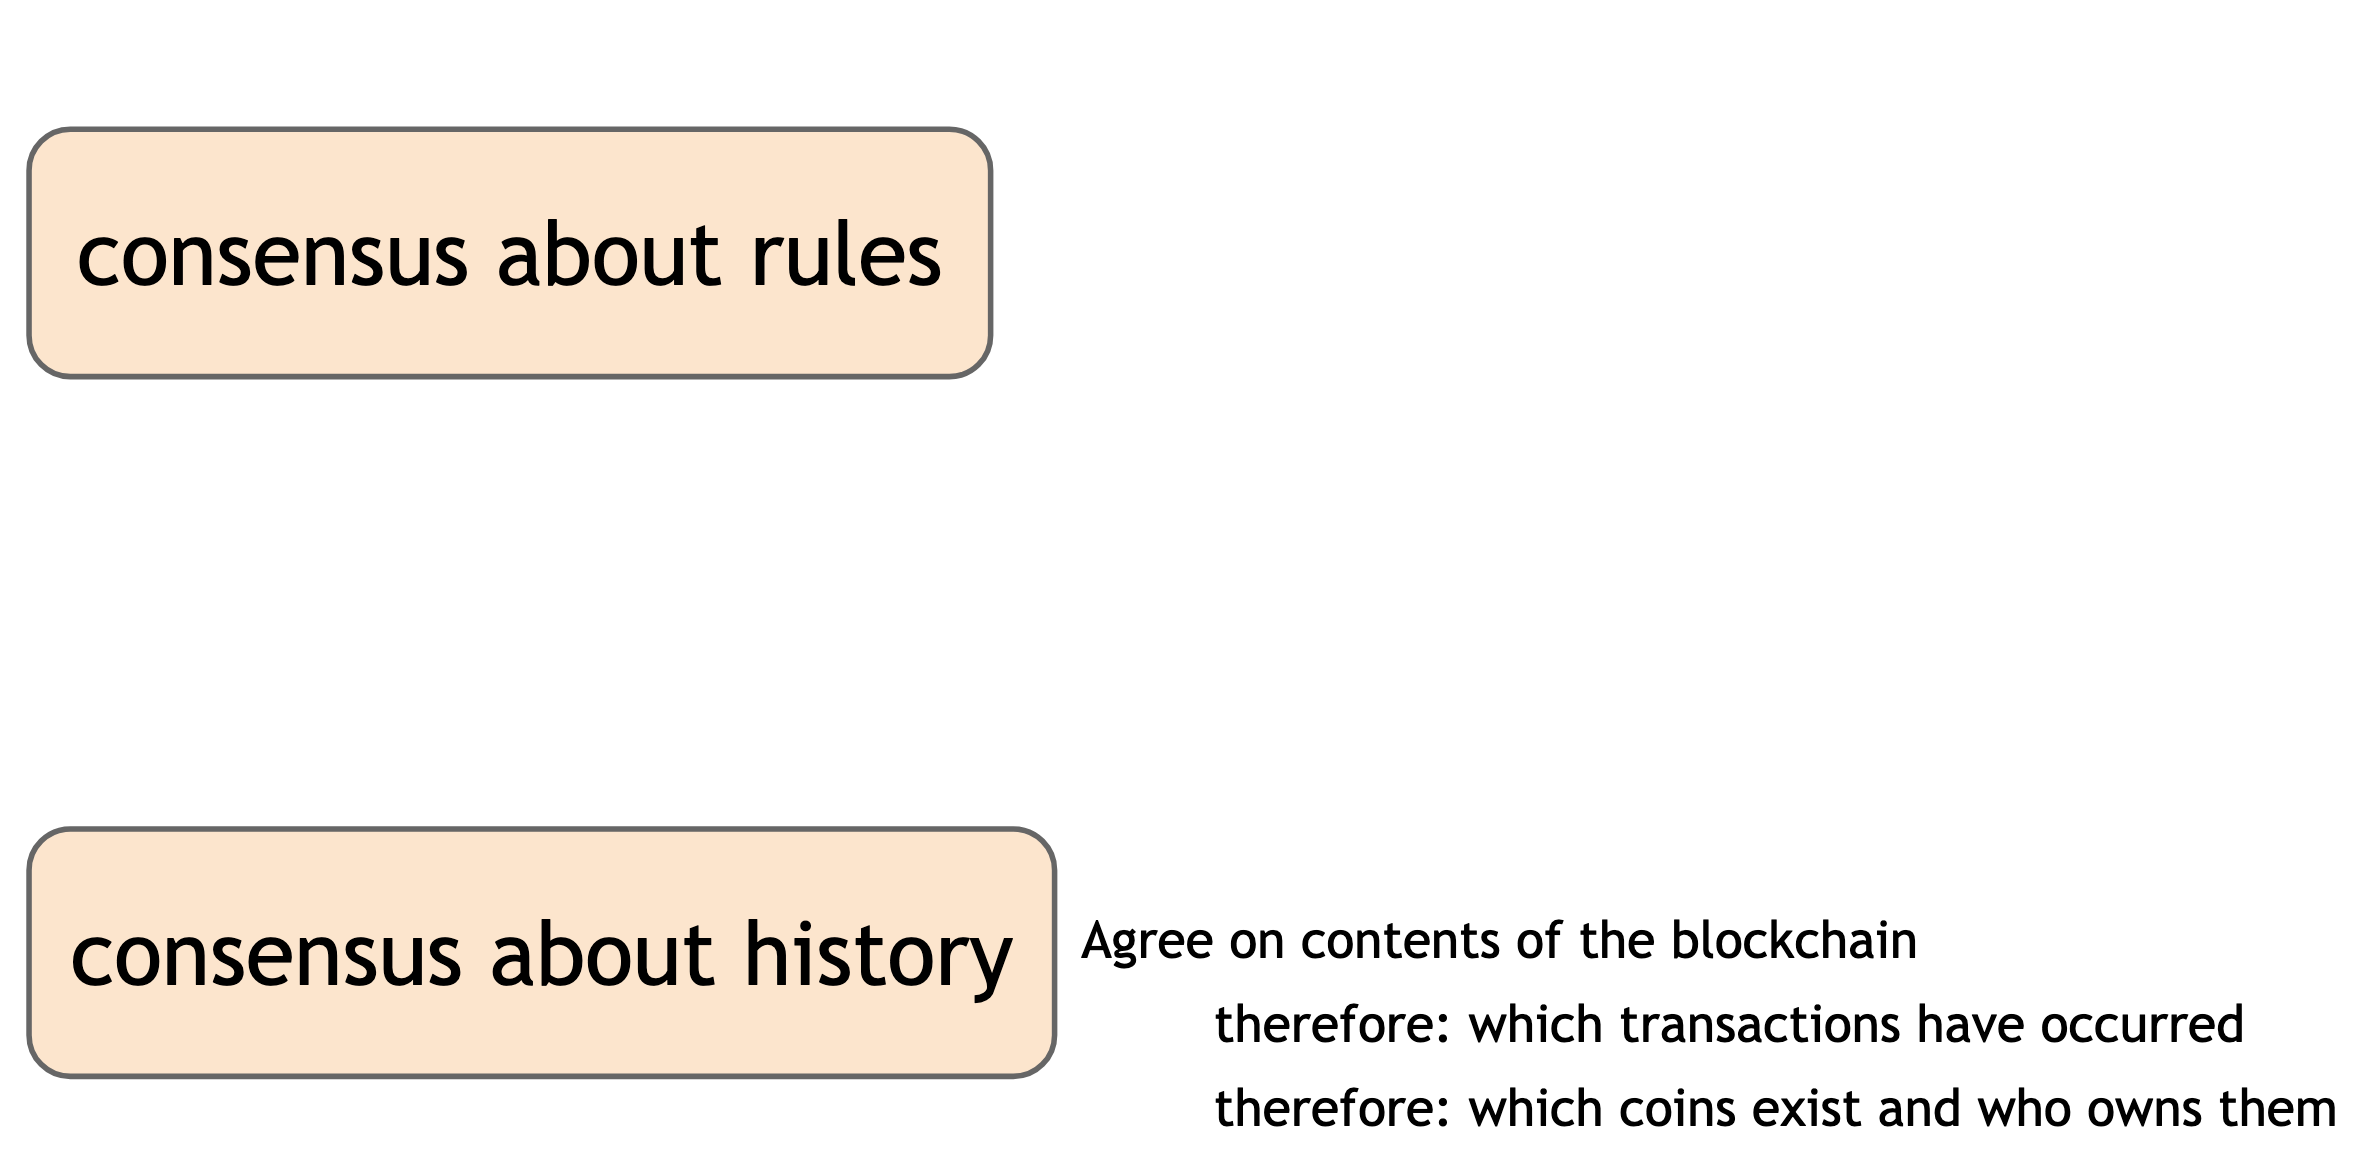
\includegraphics[scale=0.28]{history}
\end{frame}
%%%%%%%%%%%% Slide %%%%%%%%%%%%%%%%%%%%%%%%%%%%%%%%%%%%%%%%%%%%%%%%%%%
\begin{frame}
  \frametitle{Consensus in Bitcoin}
 	\centering
	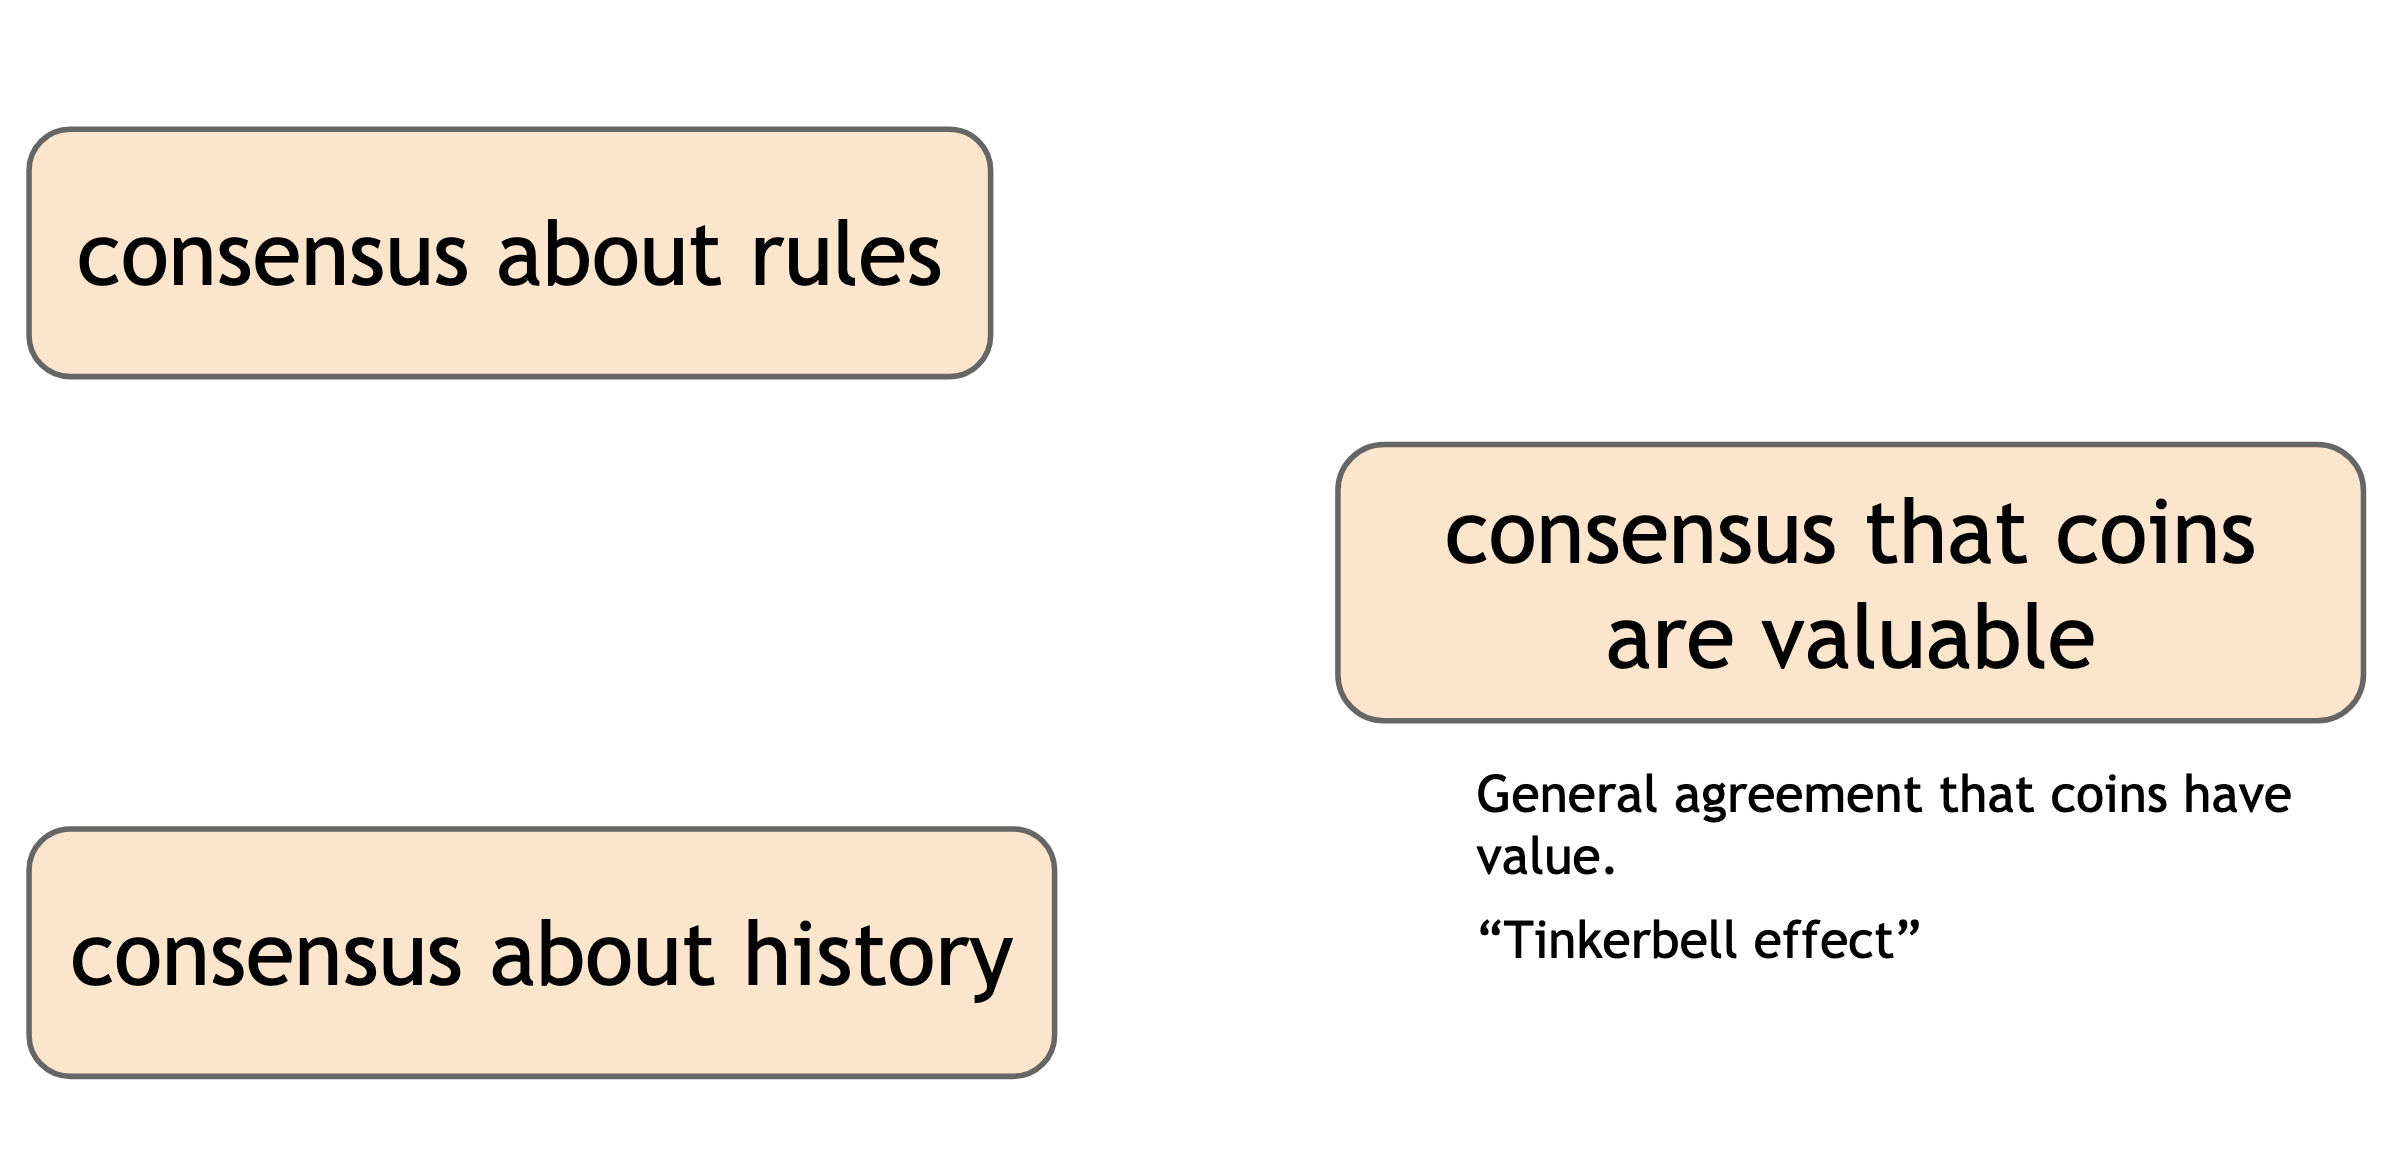
\includegraphics[scale=0.28]{value}
\end{frame}
%%%%%%%%%%%% Slide %%%%%%%%%%%%%%%%%%%%%%%%%%%%%%%%%%%%%%%%%%%%%%%%%%%
\begin{frame}
  \frametitle{Consensus in Bitcoin}
 	\centering
	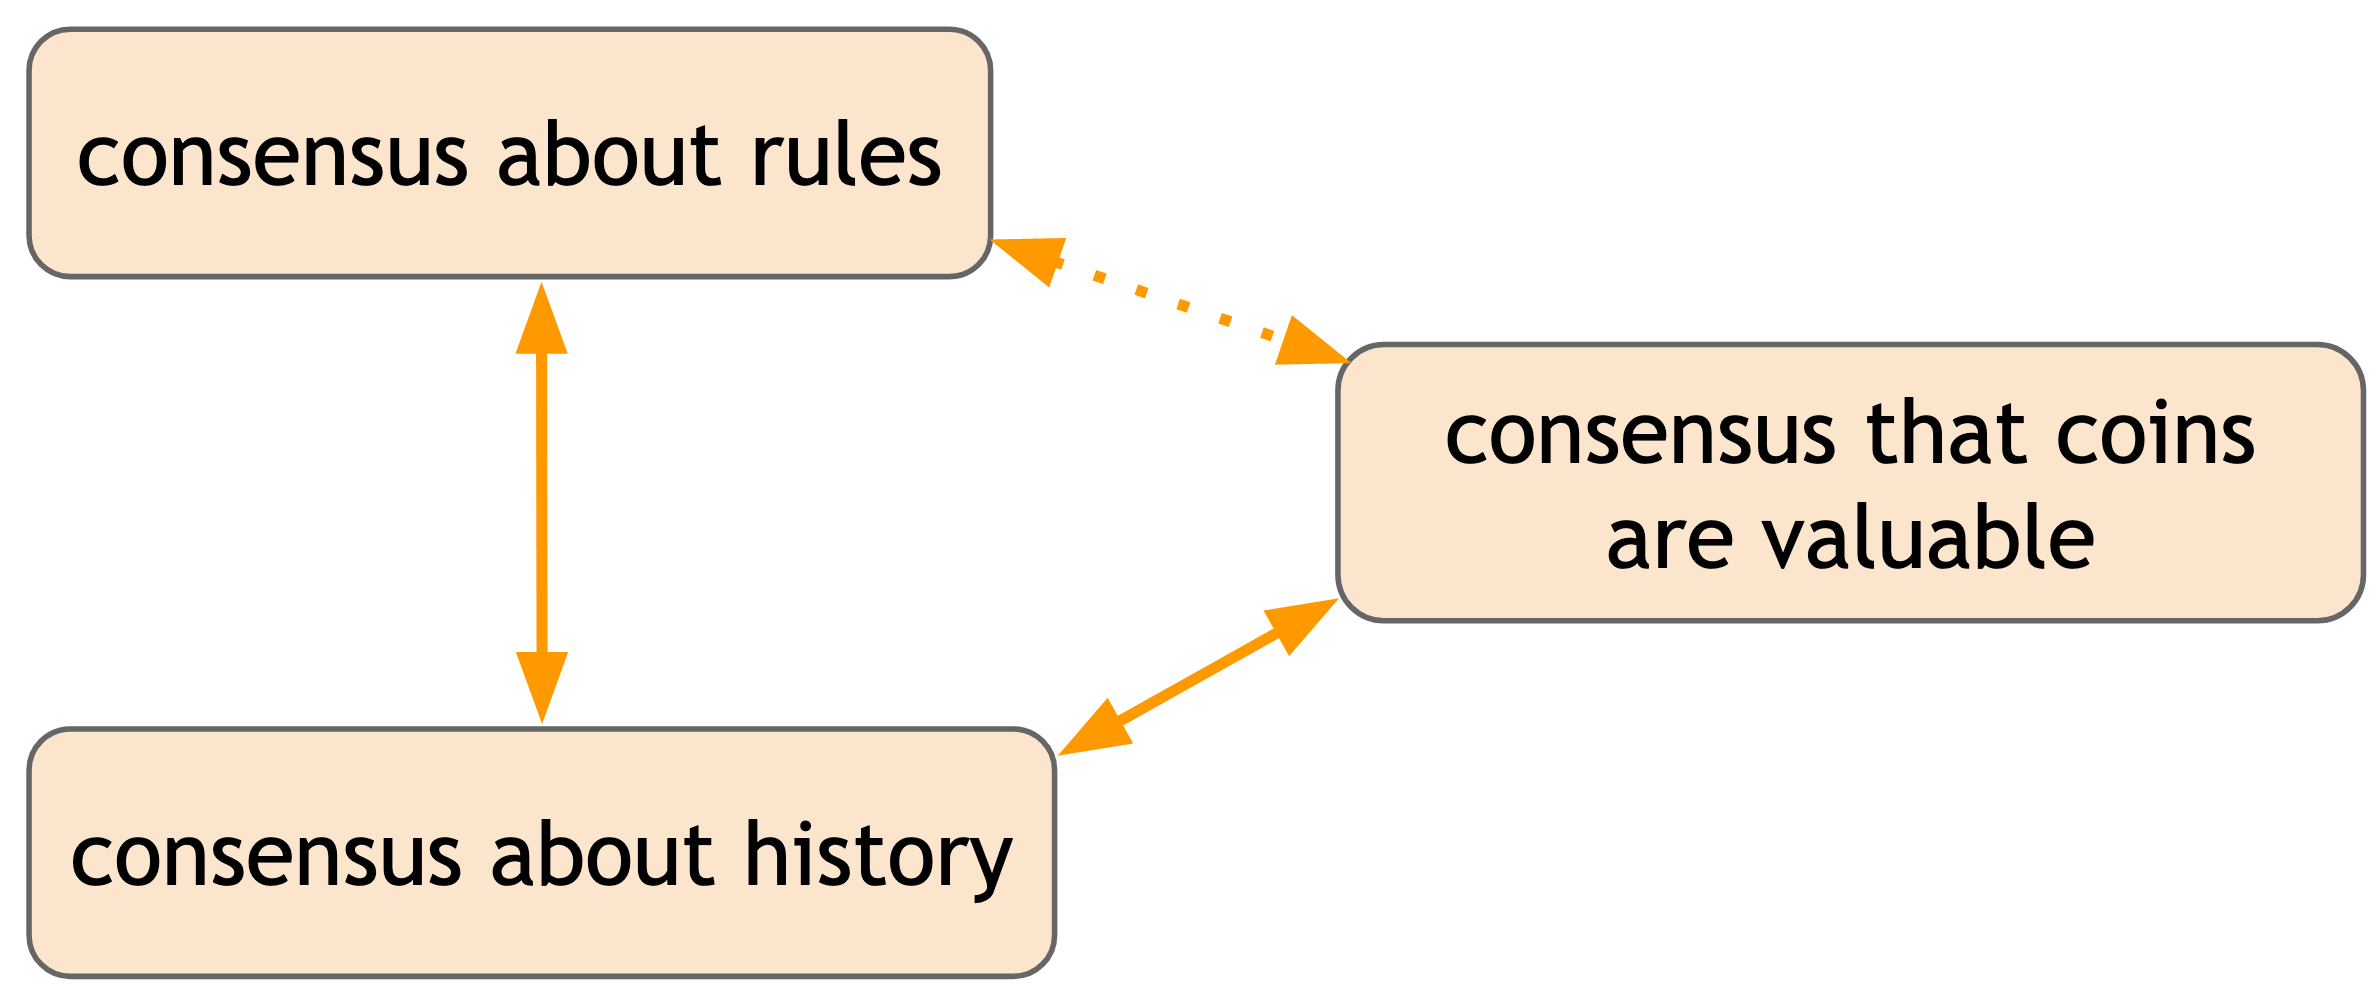
\includegraphics[scale=0.28]{all}
\end{frame}
%%%%%%%%%%%% Slide %%%%%%%%%%%%%%%%%%%%%%%%%%%%%%%%%%%%%%%%%%%%%%%%%%%
\begin{frame}
  \frametitle{Bitcoin Core Software}
  \pause
  \begin{itemize}
  	\item Open Source (MIT license).
	\item It is the de facto rule book of Bitcoin.
	\item \textcolor{brown}{Bitcoin Improvement Proposals (BIPs)}: proposal for changes to Bitcoin.
  \end{itemize}
  $ $ \\ 
  \pause
  \url{https://bitcoincore.org/}
\end{frame}
%%%%%%%%%%%% Slide %%%%%%%%%%%%%%%%%%%%%%%%%%%%%%%%%%%%%%%%%%%%%%%%%%%
\begin{frame}
  \frametitle{Users can fork the rules}
 	\centering
	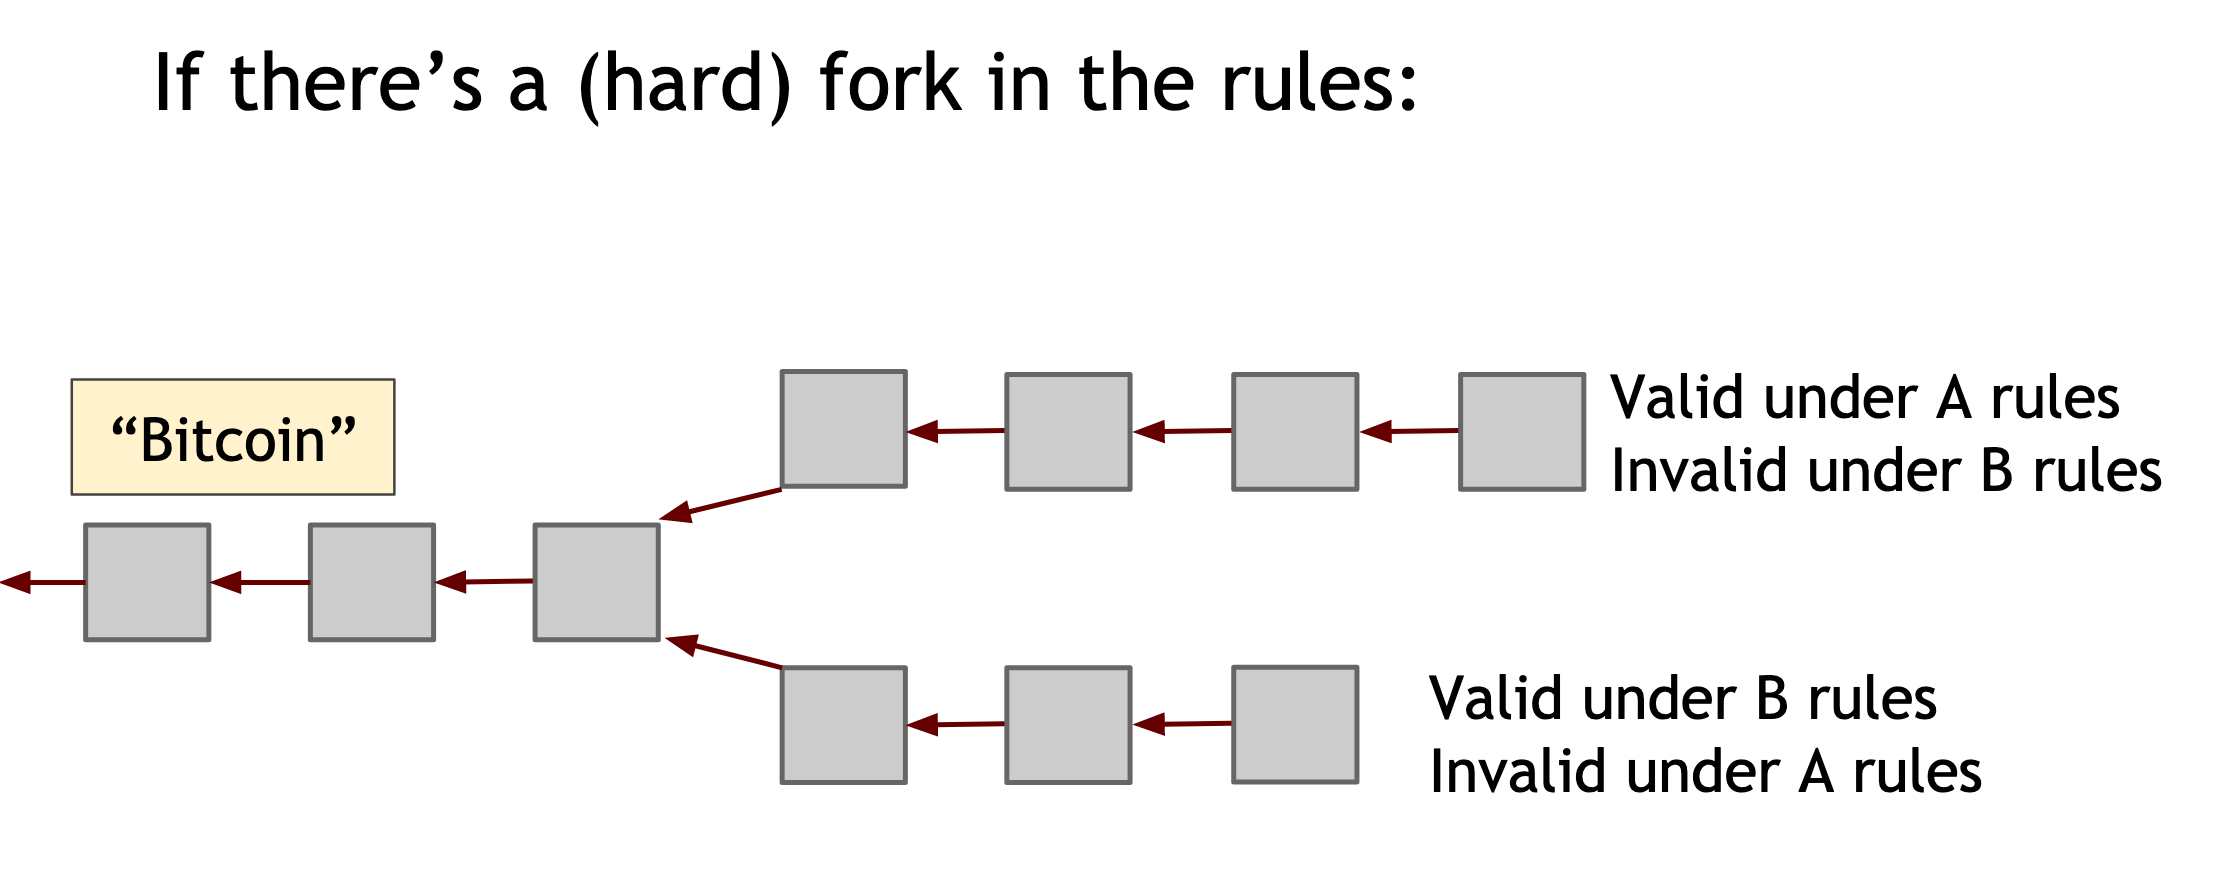
\includegraphics[scale=0.3]{fork1}
\end{frame}
%%%%%%%%%%%% Slide %%%%%%%%%%%%%%%%%%%%%%%%%%%%%%%%%%%%%%%%%%%%%%%%%%%
\begin{frame}
  \frametitle{Users can fork the rules}
 	\centering
	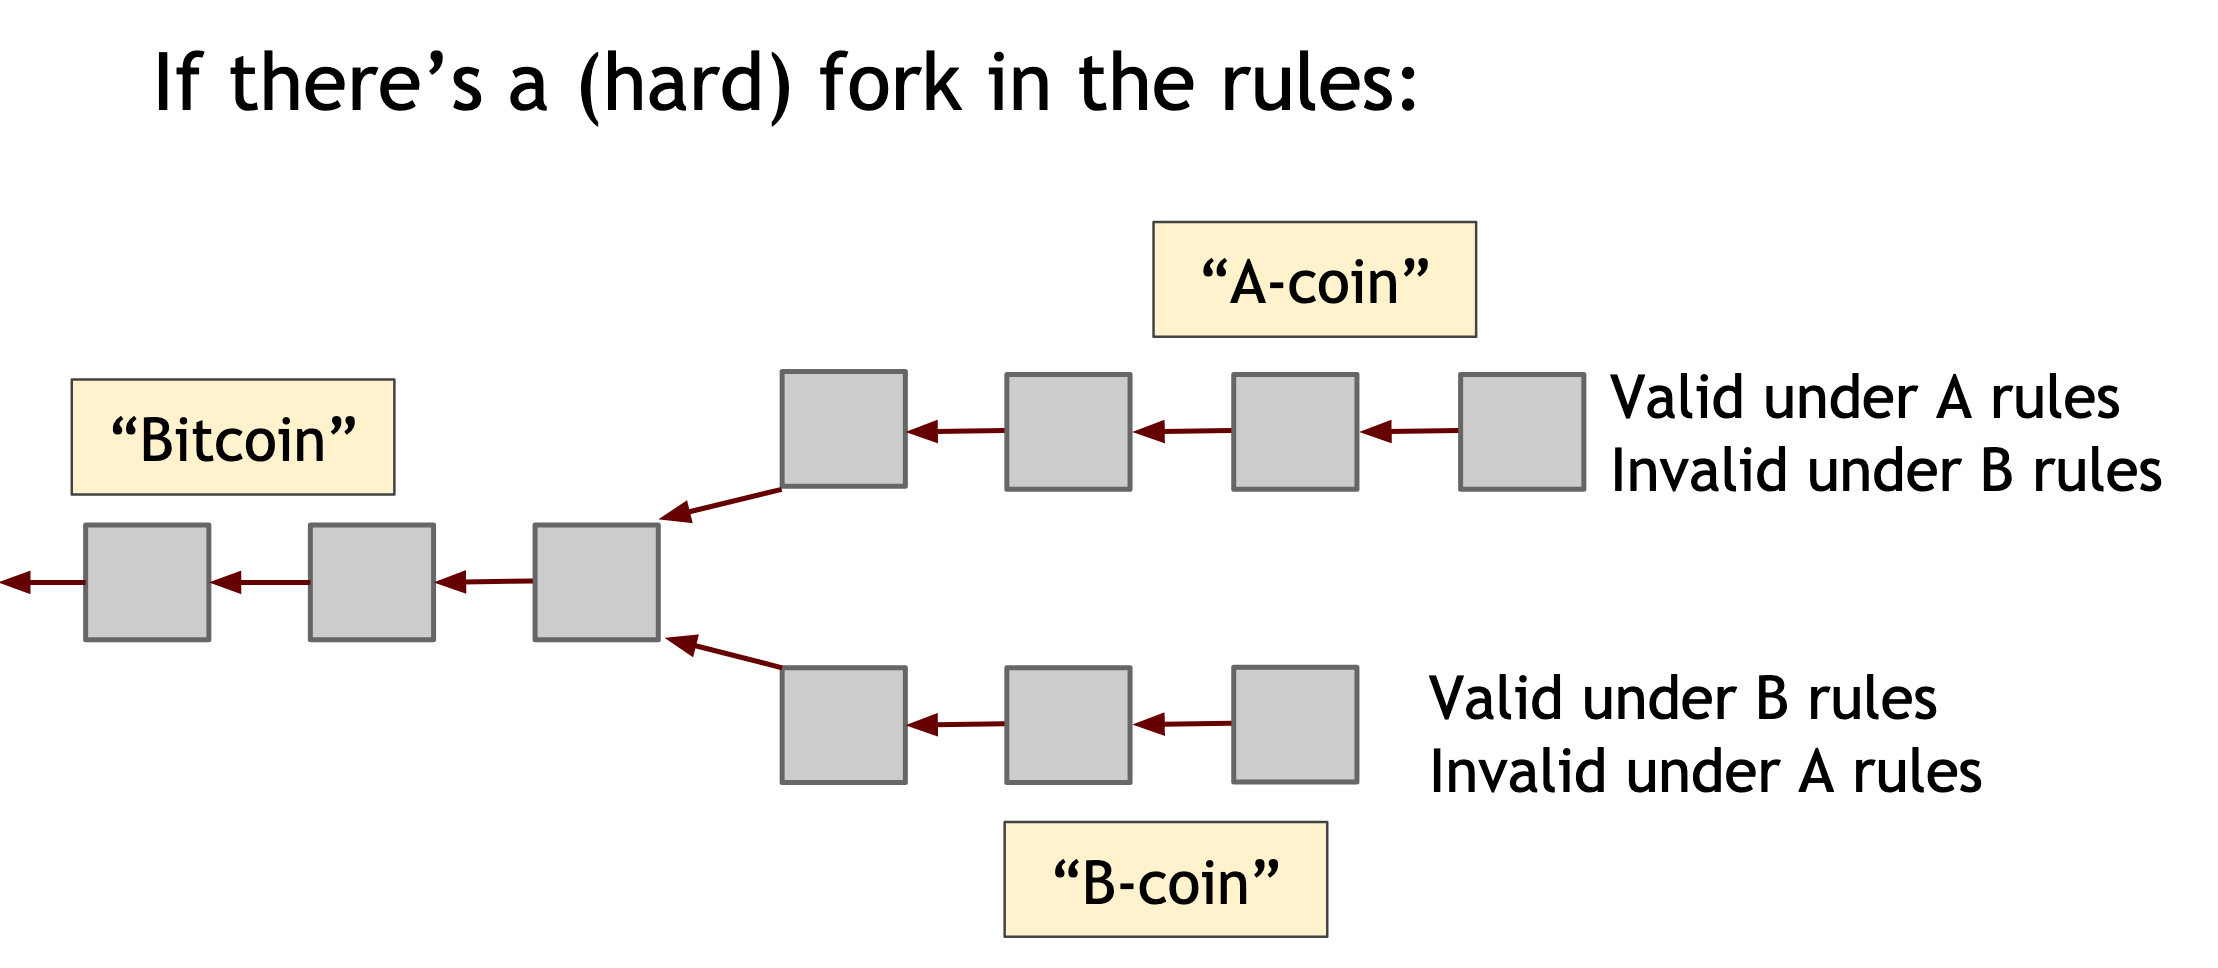
\includegraphics[scale=0.3]{fork2}
\end{frame}
%%%%%%%%%%%% Slide %%%%%%%%%%%%%%%%%%%%%%%%%%%%%%%%%%%%%%%%%%%%%%%%%%%
\begin{frame}
  \frametitle{Users can fork the rules}
 	\centering
	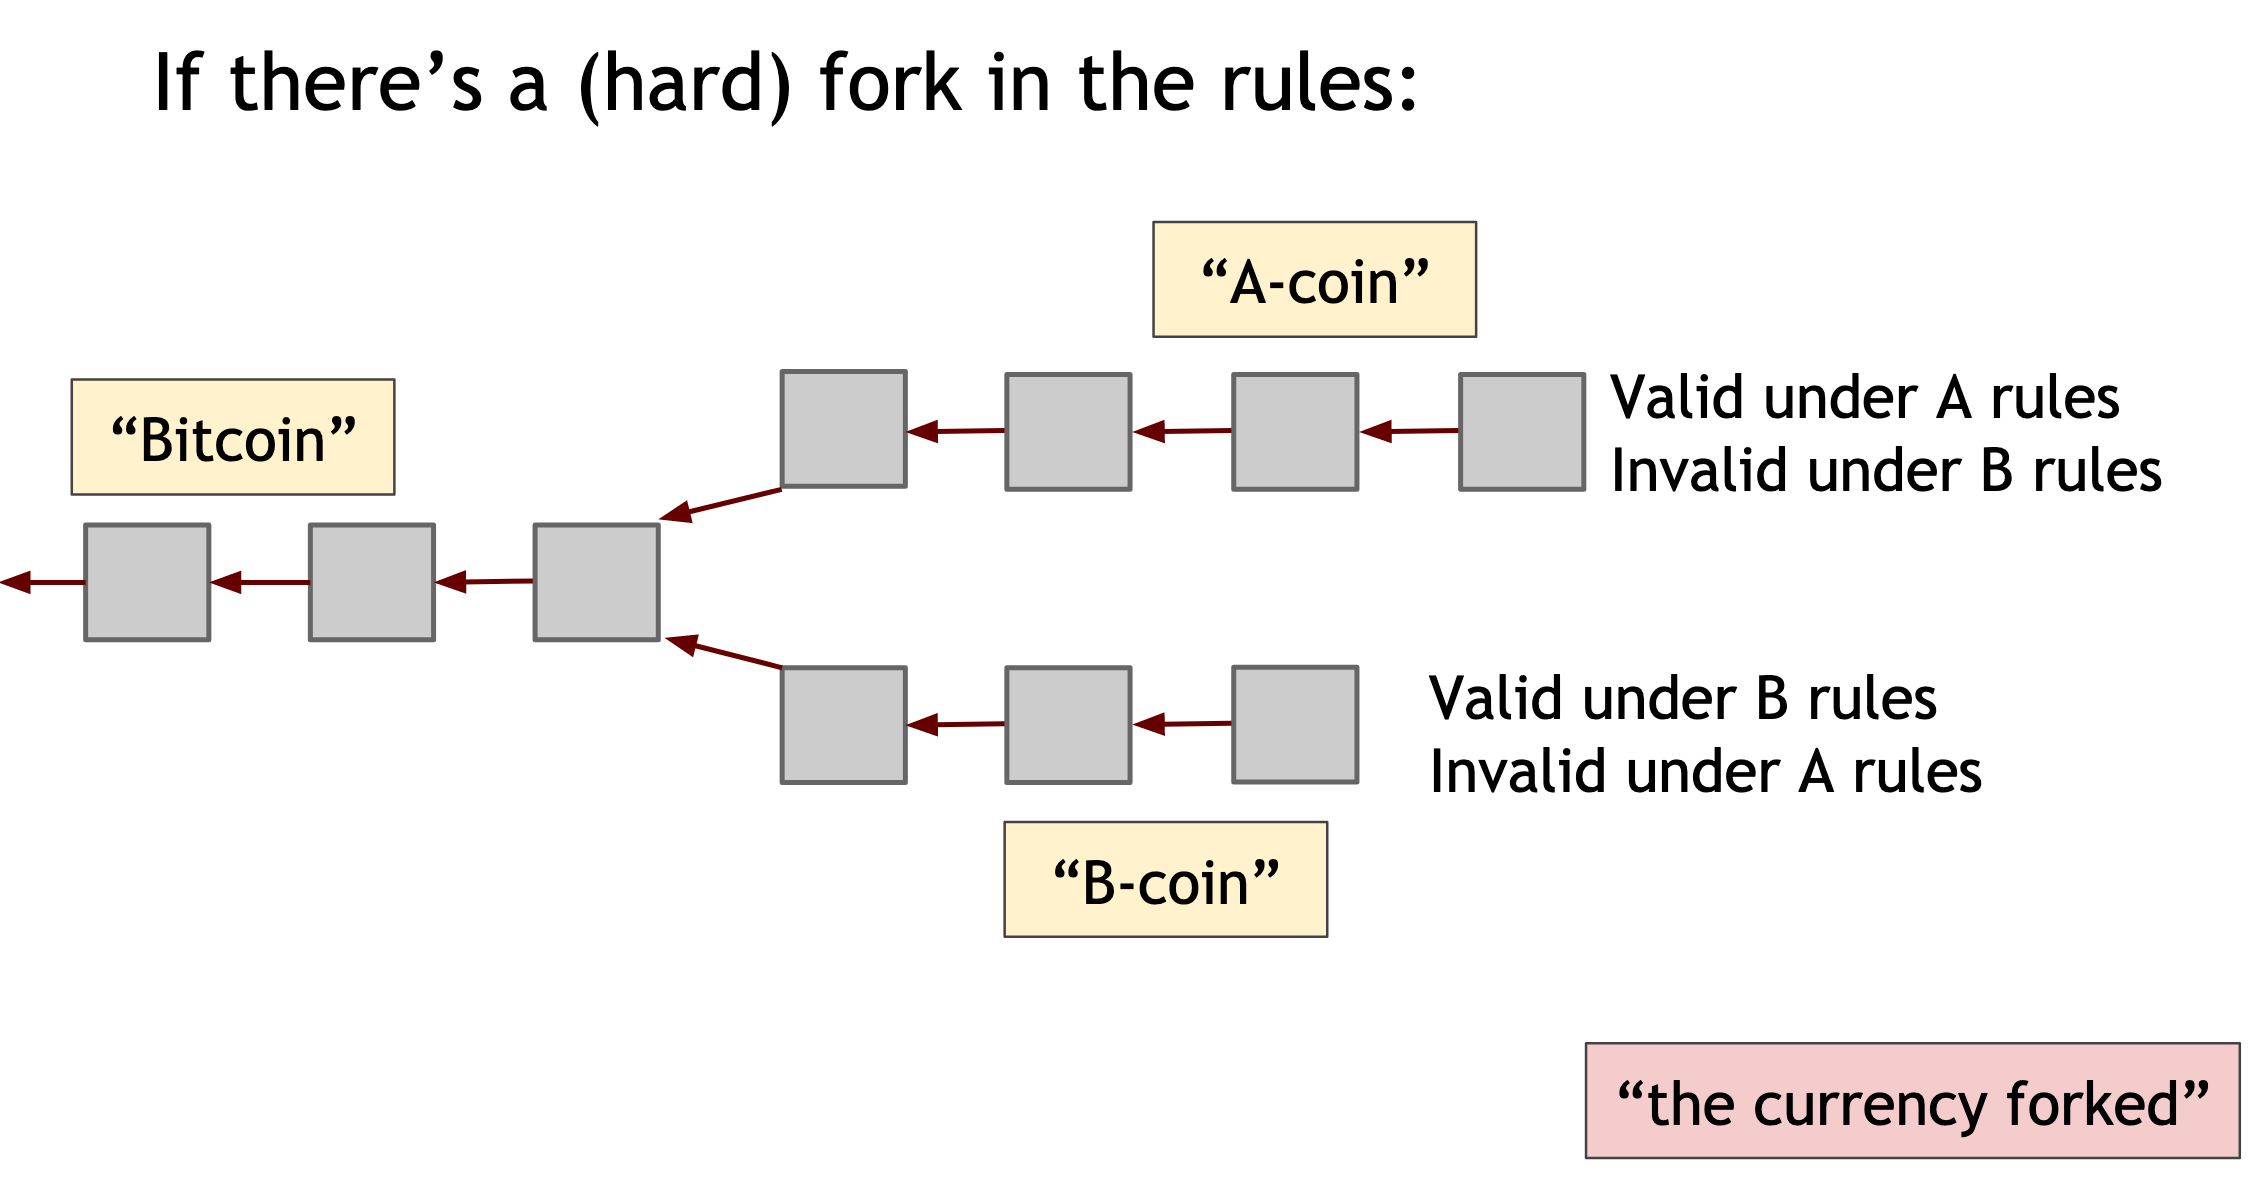
\includegraphics[scale=0.3]{fork3}
\end{frame}
%%%%%%%%%%%% Slide %%%%%%%%%%%%%%%%%%%%%%%%%%%%%%%%%%%%%%%%%%%%%%%%%%%
\begin{frame}
  \frametitle{Who has power in Bitcoin ecosystem?}
  
	\begin{itemize}
		\item \emph{Claim}: Bitcoin Core developers have the power. \pause
		\item \emph{Claim}: Miners have the power. \pause
		\item \emph{Claim}: Investors have the power. \pause
		\item \emph{Claim}: Merchants and their customers have the power. \pause
		\item \emph{Claim}: Payment services have the power.
	\end{itemize}
\end{frame}
%%%%%%%%%%%% Slide %%%%%%%%%%%%%%%%%%%%%%%%%%%%%%%%%%%%%%%%%%%%%%%%%%%
\begin{frame}
  \frametitle{Bitcoin Foundation}
  	
\includegraphics[scale=0.2]{Bitcoin-Foundation}
  	\begin{itemize}
  		\item Founded in 2012.
  		\item Pays core developers.
  		\item ``voice of Bitcoin" to governments.
  	\end{itemize}
\end{frame}

%%%%%%%%%%%% Slide %%%%%%%%%%%%%%%%%%%%%%%%%%%%%%%%%%%%%%%%%%%%%%%%%%%
\begin{frame}
  \frametitle{Governments and Bitcoin}
  
\begin{itemize}
	\item Untraceable digital cash defeats capital controls.
	\pause
	\item Untraceable digital cash makes certain kinds of crimes easier ... but \pause
	\begin{itemize}
		\item Hard to keep real and virtual separate.
   		\item Hard to stay anonymous for a long time.
    		\item Feds can ``follow the money''
	\end{itemize}
	\item \url{https://www.loc.gov/law/help/cryptocurrency/world-survey.php}
\end{itemize}
\end{frame}
%%%%%%%%%%%% Slide %%%%%%%%%%%%%%%%%%%%%%%%%%%%%%%%%%%%%%%%%%%%%%%%%%%
\begin{frame}
  \frametitle{Should Cryptocurrency be regulated?}
  \textbf{Simplified Debate!}
\begin{itemize}
	\item Arguments with examples.
	\pause
	\begin{itemize}
		\item Three arguments \textbf{for}.
		\item Three arguments \textbf{against}.
	\end{itemize}
	\item \url{https://www.loc.gov/law/help/cryptocurrency/world-survey.php}
\end{itemize}
\end{frame}

%%%%%%%%%%%% Slide %%%%%%%%%%%%%%%%%%%%%%%%%%%%%%%%%%%%%%%%%%%%%%%%%%%
\end{document}
